\begin{enunciado}{\ejercicio}
  Decidir para cada una de las siguientes matrices si los métodos de Jacobi y de Gauss-Seidel converge.
  $$
    A =
    \matriz{ccc}{
      1 & 1 & 0 \\
      -1 & 2 & 1 \\
      0 & 0 & 1 \\
    }
    \qquad
    B =
    \matriz{ccc}{
      1 & 0 & -1 \\
      -2 & 1 & 1 \\
      -1 & 0 & -1
    }
    \qquad
    C =
    \matriz{ccc}{
      3 & -1 & -4 \\
      -1 & 5 & 7 \\
      -4 & 7 & 14
    }
  $$
\end{enunciado}

\begin{enumerate}[label=\textit{Matriz} $\Alph*$:]
  \item
        $A$ es una matriz \textit{tridiagonal} es decir que averiguando el radio espectral de algún método ya
        sé lo que pasa con el otro, debido a que para este tipo de matrices:
        $$
          \rho(T_{GS}) \igual{$\llamada1$} \rho^2(T_J)
        $$
        Calculo $T_J = -D^{-1}(L+U)$:
        $$
          T_J =
          -\matriz{ccc}{
            1 & 0 & 0 \\
            0 & \frac{1}{2} & 0 \\
            0 & 0 & 1
          }
          \matriz{ccc}{
            0 & 1 & 0 \\
            -1 & 0 & 1 \\
            0 & 0 & 0
          }
          =
          \matriz{ccc}{
            0 & -1 & 0\\
            \frac{1}{2} & 0 & \frac{-1}{2}\\
            0 & 0 & 0
          } $$
        Calculo los autovalores:
        $$
          \det(T_J - \lambda I) = -\lambda \cdot (\lambda^2 + \frac{1}{2}) = 0
          \sii
          \llave{rcl}{
            \lambda_1 & = & 0\\
            \lambda_2 & = & \frac{i}{\sqrt{2}}\\
            \lambda_3 & = & \frac{-i}{\sqrt{2}}
          }
          \entonces
          \rho(T_J) = \maximo_{1\leq j \leq 3}(|\lambda_j|) = \frac{1}{\sqrt{2}} \Entonces{$\llamada1$} \rho(T_{GS}) = \frac{1}{2}
        $$
        Ambos métodos convergen dado que:
        $$
          \cajaResultado{
            \rho(T_J) = \frac{1}{\sqrt{2}} < 1 \ytext \rho(T_{GS}) \igual{\red{!}} \frac{1}{2} < 1.
          }
        $$
        En particular el método de Gauss-Seidel converge más rápido dado que el de Jacobi, dado que $\rho(T_{GS}) < \rho(T_J)$

        \bigskip

  \item
        $$
          B =
          \matriz{ccc}{
            1 & 0 & -1 \\
            -2 & 1 & 1 \\
            -1 & 0 & -1
          }
          =
          \ub{
            \matriz{ccc}{
              0 & 0 & 0 \\
              -2 & 0 & 0 \\
              -1 & 0 & 0
            }
          }{
            L
          }
          +
          \ub{
            \matriz{ccc}{
              1 & 0 & 0 \\
              0 & 1 & 0 \\
              0 & 0 & -1
            }
          }{
            D
          }
          +
          \ub{
            \matriz{ccc}{
              0 & 0 & -1 \\
              0 & 0 & 1 \\
              0 & 0 & 0
            }
          }{
            U
          }
        $$
        Puedo encontrar los autovalores de las matrices de iteración de \textit{Jacobi} y \textit{Gauss-Seidel} resolviendo las ecuaciones:
        $$
          \llamada1 ~
          \det\big(
          \blue{\lambda_J} \cdot D_J + (L_J + U_J)
          \big) = 0
          \ytext
          \llamada2 ~
          \det\big(
          \blue{\lambda_J} \cdot (D_{GS} + L_{GS}) + U_{GS}
          \big) = 0
        $$

        \bigskip

        Para $\llamada1$:
        $$
          \deter{ccc}{
            \blue{\lambda} & 0              & -1              \\
            -2             & \blue{\lambda} & 1               \\
            -1             & 0              & -\blue{\lambda}
          } = 0
          \sii
          -\blue{\lambda} \cdot (\blue{\lambda}^2 + 1) = 0
          \sii
          \llave{rcl}{
            \blue{\lambda}_1 & = & 0 \\
            \blue{\lambda}_2 & = & i \\
            \blue{\lambda}_3 & = & -i
          }
          \entonces \rho(T_J) \not< 1
          \sii
          \cajaResultado{
            \text{no converge}
          }
        $$

        \bigskip

        Para $\llamada2$:
        $$
          \deter{ccc}{
            \blue{\lambda}   & 0              & -1              \\
            -2\blue{\lambda} & \blue{\lambda} & 1               \\
            -\blue{\lambda}  & 0              & -\blue{\lambda}
          } = 0
          \sii
          -\blue{\lambda}^2 \cdot (\blue{\lambda} - 1) = 0
          \sii
          \llave{rcl}{
            \blue{\lambda}_1 & = & 0 \\
            \blue{\lambda}_2 & = & 0 \\
            \blue{\lambda}_3 & = & 1
          }
          \entonces \rho(T_{GS}) \not< 1
          \sii
          \cajaResultado{
            \text{no converge}
          }
        $$

  \item
        $C$ es una matriz \textit{simétrica y definida positiva}, porque los determinantes de sus
        menores principales son todos positivos.
        $$
          3 > 0
          ,\quad
          \deter{cc}{
            3  & -1 \\
            -1 & 5
          } = 16 > 0
          \ytext
          \deter{ccc}{
            3  & -1 & -4 \\
            -1 & 5  & 7  \\
            -4 & 7  & 14
          } = 25 > 0
        $$
        Entonces el método de \textit{Gauss-Seidel} converge.

        Puedo calcular los autovalores de $T_J$ para ver si el método de \textit{Jacobi} también lo hace:
        $$
          \deter{ccc}{
            3\blue{\lambda} & -1              & -4               \\
            -1              & 5\blue{\lambda} & 7                \\
            -4              & 7               & 14\blue{\lambda}
          } = 0
          \sii
          210 \lambda^3 - 241 \lambda + 56 = 0
        $$
        A esta altura no sé si esto está bien o no, pero bueh, llamo a ese polinomio $P$:
        $$
          P' = 0
          \sii
          630\lambda^2 - 241 = 0
          \sii
          |\lambda| \approx 0.62
        $$
        Tengo \textit{puntos críticos}, es decir posible extremos, en $ |\lambda| \approx 0.62$, y noto que la función
        \ul{crece $(\nearrow)$} en $(-\infinito, -0.62)$ y pasa de algún valor negativo, por ejemplo $P(-2)< 0$ a valores positivos en $P(1) > 0$, Bolzano y yo que sé.

        En fin hay un autovalor menor a $-1$, es decir que $|\lambda| > 1$:
        $$
          \cajaResultado{
            \rho(T_J) > 1
          }
        $$
        por lo tanto \ul{el método de \textit{Jacobi} no converge}.

        Acá te dejo un grafiquito de $P =  210 \lambda^3 - 241 \lambda + 56$: $
          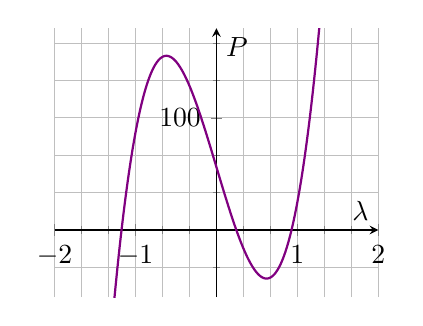
\begin{tikzpicture}[baseline = 3cm]
            \begin{axis}[scale = 0.6,
                xlabel={$\blue{\lambda}$},
                ylabel={$P$},
                grid=both,
                % grid style={gray!30},
                axis lines=middle,
                xmin=-2, xmax=2,
                ymin=-60, ymax=180,
                samples=300,
                smooth,
                % tick align=inside,
                minor tick num=2,
              ]
              \addplot[violet, thick, domain=-2:2] {210*x^3 - 241*x + 56};
            \end{axis}
          \end{tikzpicture}
        $
\end{enumerate}

\begin{aportes}
  \item \aporte{\dirRepo}{naD GarRaz \github}
\end{aportes}
